% Created by tikzDevice version 0.12.3.1 on 2022-04-16 21:51:50
% !TEX encoding = UTF-8 Unicode
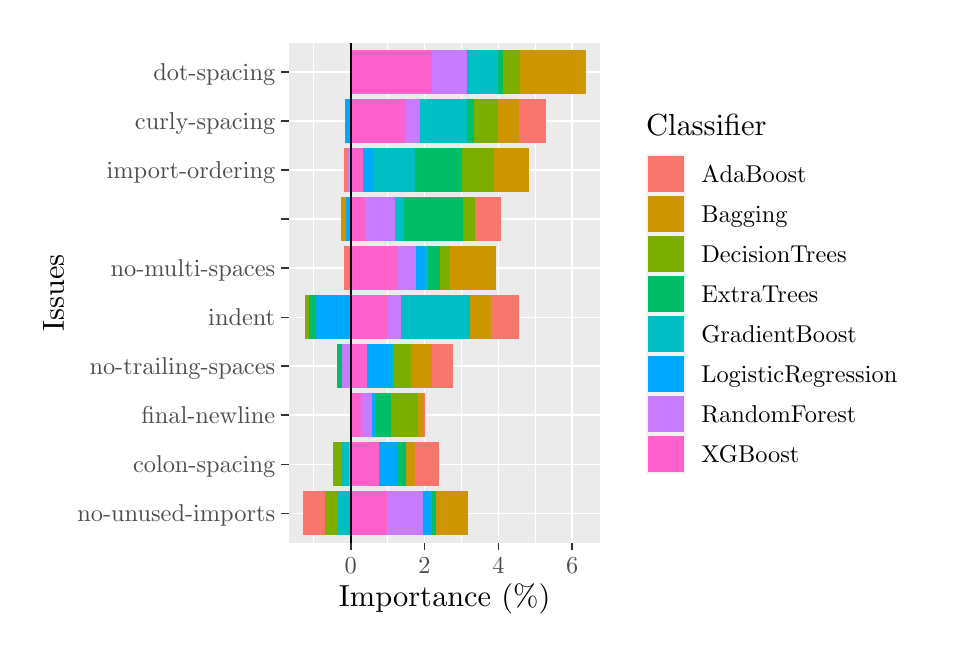
\begin{tikzpicture}[x=1pt,y=1pt]
\definecolor{fillColor}{RGB}{255,255,255}
\path[use as bounding box,fill=fillColor,fill opacity=0.00] (0,0) rectangle (325.21,216.81);
\begin{scope}
\path[clip] (  0.00,  0.00) rectangle (325.21,216.81);
\definecolor{drawColor}{RGB}{255,255,255}
\definecolor{fillColor}{RGB}{255,255,255}

\path[draw=drawColor,line width= 0.6pt,line join=round,line cap=round,fill=fillColor] (  0.00,  0.00) rectangle (325.21,216.81);
\end{scope}
\begin{scope}
\path[clip] ( 94.40, 30.69) rectangle (206.96,211.31);
\definecolor{fillColor}{gray}{0.92}

\path[fill=fillColor] ( 94.40, 30.69) rectangle (206.96,211.31);
\definecolor{drawColor}{RGB}{255,255,255}

\path[draw=drawColor,line width= 0.3pt,line join=round] (103.38, 30.69) --
	(103.38,211.31);

\path[draw=drawColor,line width= 0.3pt,line join=round] (130.07, 30.69) --
	(130.07,211.31);

\path[draw=drawColor,line width= 0.3pt,line join=round] (156.75, 30.69) --
	(156.75,211.31);

\path[draw=drawColor,line width= 0.3pt,line join=round] (183.43, 30.69) --
	(183.43,211.31);

\path[draw=drawColor,line width= 0.6pt,line join=round] ( 94.40, 41.31) --
	(206.96, 41.31);

\path[draw=drawColor,line width= 0.6pt,line join=round] ( 94.40, 59.02) --
	(206.96, 59.02);

\path[draw=drawColor,line width= 0.6pt,line join=round] ( 94.40, 76.73) --
	(206.96, 76.73);

\path[draw=drawColor,line width= 0.6pt,line join=round] ( 94.40, 94.44) --
	(206.96, 94.44);

\path[draw=drawColor,line width= 0.6pt,line join=round] ( 94.40,112.14) --
	(206.96,112.14);

\path[draw=drawColor,line width= 0.6pt,line join=round] ( 94.40,129.85) --
	(206.96,129.85);

\path[draw=drawColor,line width= 0.6pt,line join=round] ( 94.40,147.56) --
	(206.96,147.56);

\path[draw=drawColor,line width= 0.6pt,line join=round] ( 94.40,165.27) --
	(206.96,165.27);

\path[draw=drawColor,line width= 0.6pt,line join=round] ( 94.40,182.98) --
	(206.96,182.98);

\path[draw=drawColor,line width= 0.6pt,line join=round] ( 94.40,200.69) --
	(206.96,200.69);

\path[draw=drawColor,line width= 0.6pt,line join=round] (116.72, 30.69) --
	(116.72,211.31);

\path[draw=drawColor,line width= 0.6pt,line join=round] (143.41, 30.69) --
	(143.41,211.31);

\path[draw=drawColor,line width= 0.6pt,line join=round] (170.09, 30.69) --
	(170.09,211.31);

\path[draw=drawColor,line width= 0.6pt,line join=round] (196.78, 30.69) --
	(196.78,211.31);
\definecolor{fillColor}{RGB}{248,118,109}

\path[fill=fillColor] (201.45,192.72) rectangle (201.85,208.65);

\path[fill=fillColor] (177.56,175.01) rectangle (187.44,190.95);

\path[fill=fillColor] (114.32,157.30) rectangle (115.39,173.24);

\path[fill=fillColor] (161.69,139.59) rectangle (171.03,155.53);

\path[fill=fillColor] (114.19,121.88) rectangle (116.72,137.82);

\path[fill=fillColor] (167.56,104.18) rectangle (177.56,120.11);

\path[fill=fillColor] (145.94, 86.47) rectangle (153.55,102.40);

\path[fill=fillColor] (143.14, 68.76) rectangle (143.68, 84.70);

\path[fill=fillColor] (139.94, 51.05) rectangle (148.61, 66.99);

\path[fill=fillColor] ( 99.51, 33.34) rectangle (107.39, 49.28);
\definecolor{fillColor}{RGB}{205,150,0}

\path[fill=fillColor] (177.83,192.72) rectangle (201.45,208.65);

\path[fill=fillColor] (169.96,175.01) rectangle (177.56,190.95);

\path[fill=fillColor] (168.49,157.30) rectangle (181.03,173.24);

\path[fill=fillColor] (113.12,139.59) rectangle (114.86,155.53);

\path[fill=fillColor] (152.48,121.88) rectangle (169.29,137.82);

\path[fill=fillColor] (159.82,104.18) rectangle (167.56,120.11);

\path[fill=fillColor] (138.61, 86.47) rectangle (145.94,102.40);

\path[fill=fillColor] (141.01, 68.76) rectangle (143.14, 84.70);

\path[fill=fillColor] (136.60, 51.05) rectangle (139.94, 66.99);

\path[fill=fillColor] (147.68, 33.34) rectangle (159.15, 49.28);
\definecolor{fillColor}{RGB}{124,174,0}

\path[fill=fillColor] (171.83,192.72) rectangle (177.83,208.65);

\path[fill=fillColor] (161.29,175.01) rectangle (169.96,190.95);

\path[fill=fillColor] (157.02,157.30) rectangle (168.49,173.24);

\path[fill=fillColor] (157.28,139.59) rectangle (161.69,155.53);

\path[fill=fillColor] (149.15,121.88) rectangle (152.48,137.82);

\path[fill=fillColor] (100.05,104.18) rectangle (101.65,120.11);

\path[fill=fillColor] (132.47, 86.47) rectangle (138.61,102.40);

\path[fill=fillColor] (131.40, 68.76) rectangle (141.01, 84.70);

\path[fill=fillColor] (110.45, 51.05) rectangle (113.39, 66.99);

\path[fill=fillColor] (107.39, 33.34) rectangle (111.79, 49.28);
\definecolor{fillColor}{RGB}{0,190,103}

\path[fill=fillColor] (170.09,192.72) rectangle (171.83,208.65);

\path[fill=fillColor] (158.75,175.01) rectangle (161.29,190.95);

\path[fill=fillColor] (139.94,157.30) rectangle (157.02,173.24);

\path[fill=fillColor] (136.07,139.59) rectangle (157.28,155.53);

\path[fill=fillColor] (144.48,121.88) rectangle (149.15,137.82);

\path[fill=fillColor] (101.65,104.18) rectangle (104.05,120.11);

\path[fill=fillColor] (111.92, 86.47) rectangle (113.66,102.40);

\path[fill=fillColor] (125.80, 68.76) rectangle (131.40, 84.70);

\path[fill=fillColor] (133.54, 51.05) rectangle (136.60, 66.99);

\path[fill=fillColor] (146.21, 33.34) rectangle (147.68, 49.28);
\definecolor{fillColor}{RGB}{0,191,196}

\path[fill=fillColor] (159.15,192.72) rectangle (170.09,208.65);

\path[fill=fillColor] (141.81,175.01) rectangle (158.75,190.95);

\path[fill=fillColor] (124.86,157.30) rectangle (139.94,173.24);

\path[fill=fillColor] (132.60,139.59) rectangle (136.07,155.53);

\path[fill=fillColor] (143.68,121.88) rectangle (144.48,137.82);

\path[fill=fillColor] (134.74,104.18) rectangle (159.82,120.11);

\path[fill=fillColor] (131.67, 86.47) rectangle (132.47,102.40);

\path[fill=fillColor] (116.59, 68.76) rectangle (116.72, 84.70);

\path[fill=fillColor] (113.39, 51.05) rectangle (116.19, 66.99);

\path[fill=fillColor] (111.79, 33.34) rectangle (116.72, 49.28);
\definecolor{fillColor}{RGB}{0,169,255}

\path[fill=fillColor] (158.75,192.72) rectangle (159.15,208.65);

\path[fill=fillColor] (114.59,175.01) rectangle (116.72,190.95);

\path[fill=fillColor] (120.99,157.30) rectangle (124.86,173.24);

\path[fill=fillColor] (114.86,139.59) rectangle (116.72,155.53);

\path[fill=fillColor] (140.21,121.88) rectangle (143.68,137.82);

\path[fill=fillColor] (104.05,104.18) rectangle (116.72,120.11);

\path[fill=fillColor] (122.60, 86.47) rectangle (131.67,102.40);

\path[fill=fillColor] (124.33, 68.76) rectangle (125.80, 84.70);

\path[fill=fillColor] (127.00, 51.05) rectangle (133.54, 66.99);

\path[fill=fillColor] (142.74, 33.34) rectangle (146.21, 49.28);
\definecolor{fillColor}{RGB}{199,124,255}

\path[fill=fillColor] (146.21,192.72) rectangle (158.75,208.65);

\path[fill=fillColor] (136.74,175.01) rectangle (141.81,190.95);

\path[fill=fillColor] (115.39,157.30) rectangle (116.72,173.24);

\path[fill=fillColor] (121.93,139.59) rectangle (132.60,155.53);

\path[fill=fillColor] (133.67,121.88) rectangle (140.21,137.82);

\path[fill=fillColor] (130.33,104.18) rectangle (134.74,120.11);

\path[fill=fillColor] (113.66, 86.47) rectangle (116.72,102.40);

\path[fill=fillColor] (120.59, 68.76) rectangle (124.33, 84.70);

\path[fill=fillColor] (116.19, 51.05) rectangle (116.72, 66.99);

\path[fill=fillColor] (129.93, 33.34) rectangle (142.74, 49.28);
\definecolor{fillColor}{RGB}{255,97,204}

\path[fill=fillColor] (116.72,192.72) rectangle (146.21,208.65);

\path[fill=fillColor] (116.72,175.01) rectangle (136.74,190.95);

\path[fill=fillColor] (116.72,157.30) rectangle (120.99,173.24);

\path[fill=fillColor] (116.72,139.59) rectangle (121.93,155.53);

\path[fill=fillColor] (116.72,121.88) rectangle (133.67,137.82);

\path[fill=fillColor] (116.72,104.18) rectangle (130.33,120.11);

\path[fill=fillColor] (116.72, 86.47) rectangle (122.60,102.40);

\path[fill=fillColor] (116.72, 68.76) rectangle (120.59, 84.70);

\path[fill=fillColor] (116.72, 51.05) rectangle (127.00, 66.99);

\path[fill=fillColor] (116.72, 33.34) rectangle (129.93, 49.28);
\definecolor{drawColor}{RGB}{0,0,0}

\path[draw=drawColor,line width= 0.6pt,line join=round] (116.72, 30.69) -- (116.72,211.31);
\end{scope}
\begin{scope}
\path[clip] (  0.00,  0.00) rectangle (325.21,216.81);
\definecolor{drawColor}{gray}{0.30}

\node[text=drawColor,anchor=base east,inner sep=0pt, outer sep=0pt, scale=  0.88] at ( 89.45, 38.28) {no-unused-imports};

\node[text=drawColor,anchor=base east,inner sep=0pt, outer sep=0pt, scale=  0.88] at ( 89.45, 55.99) {colon-spacing};

\node[text=drawColor,anchor=base east,inner sep=0pt, outer sep=0pt, scale=  0.88] at ( 89.45, 73.70) {final-newline};

\node[text=drawColor,anchor=base east,inner sep=0pt, outer sep=0pt, scale=  0.88] at ( 89.45, 91.41) {no-trailing-spaces};

\node[text=drawColor,anchor=base east,inner sep=0pt, outer sep=0pt, scale=  0.88] at ( 89.45,109.11) {indent};

\node[text=drawColor,anchor=base east,inner sep=0pt, outer sep=0pt, scale=  0.88] at ( 89.45,126.82) {no-multi-spaces};

\node[text=drawColor,anchor=base east,inner sep=0pt, outer sep=0pt, scale=  0.88] at ( 89.45,162.24) {import-ordering};

\node[text=drawColor,anchor=base east,inner sep=0pt, outer sep=0pt, scale=  0.88] at ( 89.45,179.95) {curly-spacing};

\node[text=drawColor,anchor=base east,inner sep=0pt, outer sep=0pt, scale=  0.88] at ( 89.45,197.65) {dot-spacing};
\end{scope}
\begin{scope}
\path[clip] (  0.00,  0.00) rectangle (325.21,216.81);
\definecolor{drawColor}{gray}{0.20}

\path[draw=drawColor,line width= 0.6pt,line join=round] ( 91.65, 41.31) --
	( 94.40, 41.31);

\path[draw=drawColor,line width= 0.6pt,line join=round] ( 91.65, 59.02) --
	( 94.40, 59.02);

\path[draw=drawColor,line width= 0.6pt,line join=round] ( 91.65, 76.73) --
	( 94.40, 76.73);

\path[draw=drawColor,line width= 0.6pt,line join=round] ( 91.65, 94.44) --
	( 94.40, 94.44);

\path[draw=drawColor,line width= 0.6pt,line join=round] ( 91.65,112.14) --
	( 94.40,112.14);

\path[draw=drawColor,line width= 0.6pt,line join=round] ( 91.65,129.85) --
	( 94.40,129.85);

\path[draw=drawColor,line width= 0.6pt,line join=round] ( 91.65,147.56) --
	( 94.40,147.56);

\path[draw=drawColor,line width= 0.6pt,line join=round] ( 91.65,165.27) --
	( 94.40,165.27);

\path[draw=drawColor,line width= 0.6pt,line join=round] ( 91.65,182.98) --
	( 94.40,182.98);

\path[draw=drawColor,line width= 0.6pt,line join=round] ( 91.65,200.69) --
	( 94.40,200.69);
\end{scope}
\begin{scope}
\path[clip] (  0.00,  0.00) rectangle (325.21,216.81);
\definecolor{drawColor}{gray}{0.20}

\path[draw=drawColor,line width= 0.6pt,line join=round] (116.72, 27.94) --
	(116.72, 30.69);

\path[draw=drawColor,line width= 0.6pt,line join=round] (143.41, 27.94) --
	(143.41, 30.69);

\path[draw=drawColor,line width= 0.6pt,line join=round] (170.09, 27.94) --
	(170.09, 30.69);

\path[draw=drawColor,line width= 0.6pt,line join=round] (196.78, 27.94) --
	(196.78, 30.69);
\end{scope}
\begin{scope}
\path[clip] (  0.00,  0.00) rectangle (325.21,216.81);
\definecolor{drawColor}{gray}{0.30}

\node[text=drawColor,anchor=base,inner sep=0pt, outer sep=0pt, scale=  0.88] at (116.72, 19.68) {0};

\node[text=drawColor,anchor=base,inner sep=0pt, outer sep=0pt, scale=  0.88] at (143.41, 19.68) {2};

\node[text=drawColor,anchor=base,inner sep=0pt, outer sep=0pt, scale=  0.88] at (170.09, 19.68) {4};

\node[text=drawColor,anchor=base,inner sep=0pt, outer sep=0pt, scale=  0.88] at (196.78, 19.68) {6};
\end{scope}
\begin{scope}
\path[clip] (  0.00,  0.00) rectangle (325.21,216.81);
\definecolor{drawColor}{RGB}{0,0,0}

\node[text=drawColor,anchor=base,inner sep=0pt, outer sep=0pt, scale=  1.10] at (150.68,  7.64) {Importance (\%)};
\end{scope}
\begin{scope}
\path[clip] (  0.00,  0.00) rectangle (325.21,216.81);
\definecolor{drawColor}{RGB}{0,0,0}

\node[text=drawColor,rotate= 90.00,anchor=base,inner sep=0pt, outer sep=0pt, scale=  1.10] at ( 13.08,121.00) {Issues};
\end{scope}
\begin{scope}
\path[clip] (  0.00,  0.00) rectangle (325.21,216.81);
\definecolor{fillColor}{RGB}{255,255,255}

\path[fill=fillColor] (217.96, 50.07) rectangle (319.71,191.92);
\end{scope}
\begin{scope}
\path[clip] (  0.00,  0.00) rectangle (325.21,216.81);
\definecolor{drawColor}{RGB}{0,0,0}

\node[text=drawColor,anchor=base west,inner sep=0pt, outer sep=0pt, scale=  1.10] at (223.46,177.78) {Classifier};
\end{scope}
\begin{scope}
\path[clip] (  0.00,  0.00) rectangle (325.21,216.81);
\definecolor{fillColor}{gray}{0.95}

\path[fill=fillColor] (223.46,156.75) rectangle (237.92,171.21);
\end{scope}
\begin{scope}
\path[clip] (  0.00,  0.00) rectangle (325.21,216.81);
\definecolor{fillColor}{RGB}{248,118,109}

\path[fill=fillColor] (224.17,157.46) rectangle (237.21,170.50);
\end{scope}
\begin{scope}
\path[clip] (  0.00,  0.00) rectangle (325.21,216.81);
\definecolor{fillColor}{gray}{0.95}

\path[fill=fillColor] (223.46,142.30) rectangle (237.92,156.75);
\end{scope}
\begin{scope}
\path[clip] (  0.00,  0.00) rectangle (325.21,216.81);
\definecolor{fillColor}{RGB}{205,150,0}

\path[fill=fillColor] (224.17,143.01) rectangle (237.21,156.04);
\end{scope}
\begin{scope}
\path[clip] (  0.00,  0.00) rectangle (325.21,216.81);
\definecolor{fillColor}{gray}{0.95}

\path[fill=fillColor] (223.46,127.84) rectangle (237.92,142.30);
\end{scope}
\begin{scope}
\path[clip] (  0.00,  0.00) rectangle (325.21,216.81);
\definecolor{fillColor}{RGB}{124,174,0}

\path[fill=fillColor] (224.17,128.56) rectangle (237.21,141.59);
\end{scope}
\begin{scope}
\path[clip] (  0.00,  0.00) rectangle (325.21,216.81);
\definecolor{fillColor}{gray}{0.95}

\path[fill=fillColor] (223.46,113.39) rectangle (237.92,127.84);
\end{scope}
\begin{scope}
\path[clip] (  0.00,  0.00) rectangle (325.21,216.81);
\definecolor{fillColor}{RGB}{0,190,103}

\path[fill=fillColor] (224.17,114.10) rectangle (237.21,127.13);
\end{scope}
\begin{scope}
\path[clip] (  0.00,  0.00) rectangle (325.21,216.81);
\definecolor{fillColor}{gray}{0.95}

\path[fill=fillColor] (223.46, 98.94) rectangle (237.92,113.39);
\end{scope}
\begin{scope}
\path[clip] (  0.00,  0.00) rectangle (325.21,216.81);
\definecolor{fillColor}{RGB}{0,191,196}

\path[fill=fillColor] (224.17, 99.65) rectangle (237.21,112.68);
\end{scope}
\begin{scope}
\path[clip] (  0.00,  0.00) rectangle (325.21,216.81);
\definecolor{fillColor}{gray}{0.95}

\path[fill=fillColor] (223.46, 84.48) rectangle (237.92, 98.94);
\end{scope}
\begin{scope}
\path[clip] (  0.00,  0.00) rectangle (325.21,216.81);
\definecolor{fillColor}{RGB}{0,169,255}

\path[fill=fillColor] (224.17, 85.19) rectangle (237.21, 98.23);
\end{scope}
\begin{scope}
\path[clip] (  0.00,  0.00) rectangle (325.21,216.81);
\definecolor{fillColor}{gray}{0.95}

\path[fill=fillColor] (223.46, 70.03) rectangle (237.92, 84.48);
\end{scope}
\begin{scope}
\path[clip] (  0.00,  0.00) rectangle (325.21,216.81);
\definecolor{fillColor}{RGB}{199,124,255}

\path[fill=fillColor] (224.17, 70.74) rectangle (237.21, 83.77);
\end{scope}
\begin{scope}
\path[clip] (  0.00,  0.00) rectangle (325.21,216.81);
\definecolor{fillColor}{gray}{0.95}

\path[fill=fillColor] (223.46, 55.57) rectangle (237.92, 70.03);
\end{scope}
\begin{scope}
\path[clip] (  0.00,  0.00) rectangle (325.21,216.81);
\definecolor{fillColor}{RGB}{255,97,204}

\path[fill=fillColor] (224.17, 56.29) rectangle (237.21, 69.32);
\end{scope}
\begin{scope}
\path[clip] (  0.00,  0.00) rectangle (325.21,216.81);
\definecolor{drawColor}{RGB}{0,0,0}

\node[text=drawColor,anchor=base west,inner sep=0pt, outer sep=0pt, scale=  0.88] at (243.42,160.95) {AdaBoost};
\end{scope}
\begin{scope}
\path[clip] (  0.00,  0.00) rectangle (325.21,216.81);
\definecolor{drawColor}{RGB}{0,0,0}

\node[text=drawColor,anchor=base west,inner sep=0pt, outer sep=0pt, scale=  0.88] at (243.42,146.50) {Bagging};
\end{scope}
\begin{scope}
\path[clip] (  0.00,  0.00) rectangle (325.21,216.81);
\definecolor{drawColor}{RGB}{0,0,0}

\node[text=drawColor,anchor=base west,inner sep=0pt, outer sep=0pt, scale=  0.88] at (243.42,132.04) {DecisionTrees};
\end{scope}
\begin{scope}
\path[clip] (  0.00,  0.00) rectangle (325.21,216.81);
\definecolor{drawColor}{RGB}{0,0,0}

\node[text=drawColor,anchor=base west,inner sep=0pt, outer sep=0pt, scale=  0.88] at (243.42,117.59) {ExtraTrees};
\end{scope}
\begin{scope}
\path[clip] (  0.00,  0.00) rectangle (325.21,216.81);
\definecolor{drawColor}{RGB}{0,0,0}

\node[text=drawColor,anchor=base west,inner sep=0pt, outer sep=0pt, scale=  0.88] at (243.42,103.13) {GradientBoost};
\end{scope}
\begin{scope}
\path[clip] (  0.00,  0.00) rectangle (325.21,216.81);
\definecolor{drawColor}{RGB}{0,0,0}

\node[text=drawColor,anchor=base west,inner sep=0pt, outer sep=0pt, scale=  0.88] at (243.42, 88.68) {LogisticRegression};
\end{scope}
\begin{scope}
\path[clip] (  0.00,  0.00) rectangle (325.21,216.81);
\definecolor{drawColor}{RGB}{0,0,0}

\node[text=drawColor,anchor=base west,inner sep=0pt, outer sep=0pt, scale=  0.88] at (243.42, 74.23) {RandomForest};
\end{scope}
\begin{scope}
\path[clip] (  0.00,  0.00) rectangle (325.21,216.81);
\definecolor{drawColor}{RGB}{0,0,0}

\node[text=drawColor,anchor=base west,inner sep=0pt, outer sep=0pt, scale=  0.88] at (243.42, 59.77) {XGBoost};
\end{scope}
\end{tikzpicture}
